\chapter[DFT]{Density Functional Theory}
\section[ITRO. DFT (SHOLL)]{Introducción a la teoría DFT [\emph{Sholl}]}

La teoría DFT o \emph{Teoría de Densidad del Funcional} está basada en dos bucles auto consistentes.
\begin{enumerate}
    \item En el primer bucle, se busca la \textbf{densidad electrónica más estable} para determinar la configuración atómica.
    \item En el siguiente bucle, se busca la configuración atómica que \textbf{minimice la energía total del sistema}.
\end{enumerate}
Pueden llegar a ocurrir diferentes cosas: 
\begin{itemize}
    \item Se llegan a diferentes configuraciones finales del sistema con la misma energía. La más estable de ellas será la que aceptemos.
    \item Puede ocurrir que una configuración atómica dada tenga diferentes mínimos de energía estables. En esos casos, aparecen \textbf{dominios} en el material (que es el origen, por ejemplo, de los dominios magnéticos de un ferromagnético).
\end{itemize}

La característica fundamental de esta teoría es que se tratará a los electrones como \textbf{densidades}, $n(\B{r})$ o $\rho(\B{r})$ (dependiendo del libro). Estas densidades se definen\footnote{Una definición más acertada tendría en cuenta un factor 2 multiplicando debido al \emph{espín}: $$n(\B{r}) = \textcolor{red}{2}\sum_i \psi_i(\B{r})^* \psi_i(\B{r})$$} en términos de las funciones de onda de electrones independientes, $\{\psi_i\}$: 
\begin{equation}
    \rho(\B{r})\equiv n(\B{r}):=\sum_i |\psi_i(\B{r})|^2 = \sum_i \psi_i(\B{r})^* \psi_i(\B{r})
\end{equation}
Esta teoría esta basada en dos teoremas fundamentales de \emph{Hohenberg} y \emph{Kohn}. El primero enuncia que la densidad electrónica determina \emph{completamente} la energía del estado fundamental. Dicho de otra forma, \textbf{la energía del estado fundamental es un funcional dependiente únicamente de la densdiad electrónica}, es decir, $E\equiv E[n(\B{r})]$. Este es un resultado fundamental ya que permite reducir considerablemente la dimensionalidad del problema, pasando de considerar $N$ átomos en nuestra red a centrarnos únicamente en nuestra densidad electrónica, de tres dimensiones espaciales. No obstante, con este teorema únicamente no tenemos ninguna información sobre la forma de esa densidad $n(\B{r})$, por ello la necesidad del segundo teorema. \\

En el segundo teorema, se establece que \textbf{la densidad electrónica real} que representa a nuestro sistema es aquella que \textbf{minimiza la energía} (del estado fundamental). Esto implica que si conociésemos la relación funcional real de la densidad electrónica, podríamos variarla hasta encontrar la que minimiza la energía.\\

El siguiente paso es aproximar. Una aproximación útil (y en la cual permaneceremos a lo largo del proyecto) es en la de \textbf{electrones libres}, es decir, sin interacciones entre ellos. De esta manera, se puede llegar a un funcional de la energía aproximado dado por
\begin{equation} \label{1.1}
    E[\{ \psi_i \}] = E_\text{conocido}[\{ \psi_i \}] + E_\text{XC}[\{ \psi_i \}] \ .
\end{equation}
\begin{itemize}
    \item El término $E_\text{conocido}[\{ \psi_i \}]$ corresponde a los términos que conocemos analíticamente, que son las energías cinéticas de los electrones (KE), interacciones electrón-núcleo, electrón-electrón y núcleo-núcleo de tipo coulombianas (EN, EE y NN, respectivamente).
    \begin{equation}
        E_\text{conocida}[\{ \psi_i \}]=\underbrace{-\frac{\hbar^2}{2m} \sum\nolimits_i \int \psi_i^* \laplacian \psi_i \D[3]{r}}_{\text{KE}} + \underbrace{\int V(\B{r})n(\B{r}) \D[3]{r}}_{\text{EN}} + \underbrace{\frac{e^2}{2}\iint \frac{n(\B{r})n(\B{r'})}{|\B{r}-\B{r'}|} \D[3,3]{r,r'}}_{\text{EE}} + E_\text{NN}
    \end{equation}

    \item El término $E_\text{XC}[\{ \psi_i \}]$ corresponde al funcional de correlación-canje, que incluye el resto de efectos mecano-cuánticos no tenidos en cuenta. De momento no tenemos nada de información sobre él.
\end{itemize}

Suponiendo que conozcamos la forma funcional del término de canje-correlación, necesitamos una manera de encontrar las funciones de onda $\{\psi_i\}$ de manera sencilla. Esto se consigue resolviendo las \emph{ecuaciones de Kohn-Sham}, que reducen esta tarea laboriosa a resolver la ecuación de Schrödinger para un solo electrón.
\begin{equation}
    \left [-\frac{\hbar^2}{2m}\laplacian +V(\B{r}) + V_H(\B{r}) + V_\text{XC}(\B{r}) \right ]\psi_i(\B{r}) = \varepsilon_i\psi_i(\B{r})
\end{equation}
\begin{itemize}
    \item El potencial $V(\B{r})$ corresponde a la interacción entre un electrón y el conjunto de los núcleos atómicos.
    \item El potencial $V_H(\B{r})$ se conoce como \textbf{potencial de Hartree}, definido como:
    $$
     V_H(\B{r})=e^2\int \frac{n(\B{r'})}{|\B{r}-\B{r'}|} \D[3]{r'} \ .
    $$
    Describe la interacción de repulsión coulombiana entre el electrón considerado y el conjunto de electrones dentro de la densidad electrónica. Como el electrón considerado también pertenece a $n(\B{r})$, este potencial describe una auto-repulsión hacia el electrón. Para corregir esa auto-repulsión, se añade un término correspondiente dentro de $V_\text{XC}$.

    \item El potencial $V_\text{XC}$ describe las contribuciones de correlación-canje {\scriptsize (lol gracias sara)}. Puede expresarse formalmente como una  \emph{derivada funcional} \footnote{Más información de derivadas funcionales: \url{https://es.wikipedia.org/wiki/Derivada_funcional} .}:
    $$
    V_\text{XC}(\B{r}) = \fdv{E_\text{XC}}{n(\B{r})}
    $$
\end{itemize}

Para calcular la función de onda del electrón necesitamos la densidad electrónica, pero para calcular la densidad electrónica necesitamos la función de onda del electrón. El cálculo es circular, pero una manera de solventarlo es implementar un método iterativo, que es en donde entra en juego el primer bucle auto consistente que mencionábamos al principio.

\newpage

\section[INTRO. DFT (FOR BEGINNERS)]{Introducción a la DFT [\emph{DFT for beginners}]}
De la misma manera, partimos de la \emph{ecuación de Schrödinger}
\begin{equation}
    \hat{H}_S \Phi\left ( \{ \B{r}_i \} , \{ \B{R}_\alpha  \} \right ) = E_\text{TOT} \Phi \left ( \{ \B{r}_i \} , \{ \B{R}_\alpha  \} \right )
\end{equation}
donde $\{ \B{r}_i\}$ y $\{ \B{R}_\alpha\}$ son las coordenadas de los electrones y de los iones, respectivamente. El hamiltoniano es:
\begin{equation}
    \hat{H}_S = \sum _\alpha \frac{P_\alpha ^2}{2M_\alpha } + \sum _i \frac{p_i^2}{2m_i} + \frac{1}{2} \sum_{i\neq j} \frac{1}{|\B{r}_i - \B{r}_j |} - \sum _{i,\alpha } \frac{Z_\alpha }{|\B{r}_i - \B{R}_\alpha |} + \frac{1}{2} \sum_{\alpha \neq \beta } \frac{Z_\alpha Z_\beta }{|\B{R}_\alpha - \B{R}_\beta |}
\end{equation}
\subsection{1ª aproximación: Born-Oppenheimer (electrones independientes)}
Separamos el movimiento electrónico del iónico.
\begin{equation}
    \left ( \hat{H}_S - \sum_\alpha \frac{P_\alpha ^2}{2M_\alpha } \right ) \Psi_{\{ \B{R}_\alpha  \} } (\{ \B{r}_i \}) = E_\text{fund}(\{ \B{R}_\alpha  \}) \Psi {\{ \B{R}_\alpha  \} } (\{ \B{r}_i \})
\end{equation}
La energía total se convierte en
\begin{equation}
    E_\text{TOT} = \sum_\alpha \frac{P_\alpha ^2}{2M_\alpha } + E_\text{fund} (\{ \B{R}_\alpha  \})\ .
\end{equation}
Las fuerzas que actúan sobre los iones son :
\begin{equation}
    \B{F}_\beta = -\pdv{E_\text{fund}}{\B{R}_\beta } \ (\{ \B{R}_\alpha  \})
\end{equation}
\subsection{2ª aproximación: Hohenberg-Kohn}
Los electrones pasan a representarse mediante densidades electrónicas.
$$
e^- \longrightarrow \rho(\B{r}) = N_e \int \left | \Psi \left (\{ \B{r}_i \}_{i=1}^N  \right ) \right |^2 \D{\B{r}_1}\ldots \D{\B{r}_N}
$$
\subsection{3ª aproximación: [2º Teorema de Hohenberg-Kohn]}
Los potenciales de la forma $v(\B{r})=\sum_\alpha -Z_\alpha /|\B{r}-\B{R}_\alpha |$ presentan funcionales \textbf{únicos} de densidades electrónicas:
\begin{equation}
    E\equiv E[\rho(\B{r})]
\end{equation}
Esto lleva a definir la energía fundamental como:
\begin{equation}
    E_\text{fund} = E[\rho_\text{fund}] + \frac{1}{2} \sum _{\alpha \neq \beta } \frac{Z_\alpha Z_\beta }{|\B{R}_\alpha - \B{R}_\beta |}
\end{equation}
\subsection{4ª aproximación: Ecuaciones de Kohn-Sham}
El problema de resolver N ecuación de Schrödinger puede simplificarse a resolver una única ecuación de un electrón independiente:
\begin{equation}
    E[\rho] = \int v(\B{r}) \rho (\B{r}) \D{\B{r}} + E_{ee}[\rho] + T_S [\rho] + E_{XC} [\rho]
\end{equation}
\begin{itemize}
    \item $E_{ee}$ es la energía de interacción (coulombiana) electrón-electrón:
    $$
    E_{ee} := \frac{1}{2} \iint \frac{\rho(\B{r}) \rho(\B{r}')}{|\B{r} - \B{r}'|} \D{\B{r},\B{r}'}
    $$

    \item $T_S[\rho] $ es la energía cinética de electrones no interactuantes entre sí, para $\rho(\B{r}) = \sum_{n=1} ^{N_e} |\psi_n(\B{r})|^2$ . 
    \begin{equation*}
        \begin{split}
                \left [ -\frac{1}{2}\laplacian + V(\B{r}) \right ] \psi_n (\B{r}) &= \varepsilon_n \psi_n (\B{r})\\
                                                                        T_S[\rho] &= \sum_{n=1} ^{N_e} \varepsilon_n - \int V(\B{r}) \rho (\B{r}) \D{\B{r}}                                \\
                                                                         V(\B{r}) &= v(\B{r}) + \int \frac{\rho(\B{r}')}{|\B{r}-\B{r}'|} \D{\B{r}'} + \fdv{E_{XC}}{\rho }\\
                                                                                  &= v(\B{r}) + V_H(\B{r}) + V_{XC}(\B{r})
        \end{split}
    \end{equation*}
\end{itemize}
Observamos que para obtener los orbitales electrónicos, necesitamos la densidad electrónica; pero para obtener la densidad electrónica, necesitamos los orbitales electrónicos. Para encontrar ambos, creamos un bucle auto consistente y la densidad de estados en cada iteración se convierte en una combinación de la de entrada y salida del bucle.
\begin{figure}[h!]
    \centering
    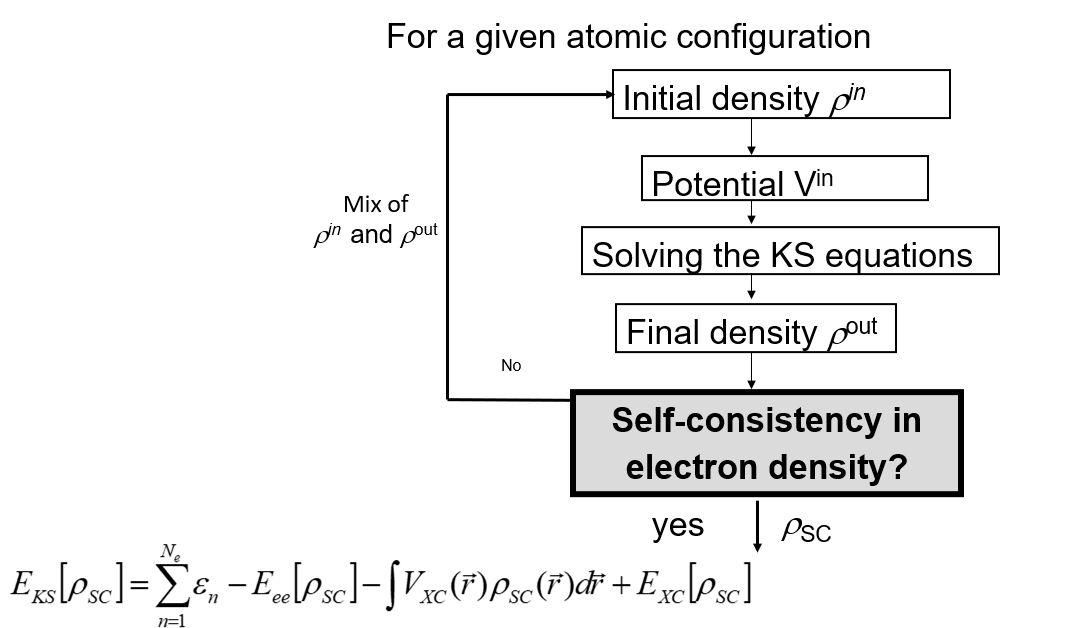
\includegraphics[scale=.4]{FIGURAS/bucle dft.png}
    \label{fig:bucle}
\end{figure}

\subsection{Otras aproximaciones}
\begin{itemize}
    \item \textbf{Aproximación de pseudo-potencial: } Bajo esta aproximación, los electrones de capas más internas se integran con el núcleo y se toman en cuenta únicamente las contribuciones a enlaces de los electrones de la capa de valencia. Esto reduce el número de variables a tener en cuenta en el cálculo.

    \item \textbf{Correlación y canje: }Para modelar el término de correlación y canje se pueden llevar a cabo diferentes tipos de aproximaciones, siendo la más sencilla la LDA (\emph{Local Density Approximation}). Según el modelo LDA, la energía en un punto $r$ corresponde a la energía de un gas electrónico homogéneo con la misma densidad electrónica en ese punto.
    \begin{equation*}
        \begin{split}
            E_{XC}{}^{(LDA)}[\rho ]&=\int \varepsilon_{XC} (\rho) \rho(\B{r}) \D{r} \implies V_{XC}{}^{(LDA)}=\pdv{[\rho(\B{r})\varepsilon_{XC}(\rho)]}{\rho(\B{r})}\\
            \varepsilon_{XC} &= \varepsilon_{XC}{}^\text{hom}[\rho]
        \end{split}
    \end{equation*}

    \item \textbf{Aproximación ión-ión: enfoque de Ewald.} Para lidiar con la suma de infinitos términos en el término de interacción ión-ión, se introduce un parámetro $\eta$ para hacer converger rápidamente la suma.
\end{itemize}